\documentclass[conference]{IEEEtran}

\usepackage[utf8]{inputenc}
\usepackage[T1]{fontenc}
\usepackage[brazil]{babel}
\usepackage{graphicx}
\usepackage{booktabs}
\usepackage{amsmath}
\usepackage{url}
\usepackage{xcolor}
\usepackage{array}
\usepackage{textcomp}
\usepackage{placeins}
\usepackage{tikz}
\usetikzlibrary{positioning,arrows.meta}
\usepackage{listings}
\usepackage[hidelinks]{hyperref}

\newcolumntype{L}[1]{>{\raggedright\arraybackslash}p{#1}}
\emergencystretch=1.5em

\graphicspath{{figuras/}}

% permite mais figuras por coluna, para ficarem perto do texto
\renewcommand{\topfraction}{0.9}
\renewcommand{\bottomfraction}{0.7}
\renewcommand{\textfraction}{0.08}
\renewcommand{\floatpagefraction}{0.85}
\setcounter{topnumber}{3}
\setcounter{bottomnumber}{2}
\setcounter{totalnumber}{4}

\lstset{
  language=Python,
  basicstyle=\ttfamily\scriptsize,
  keywordstyle=\color{blue!70!black}\bfseries,
  commentstyle=\color{gray}\itshape,
  stringstyle=\color{orange!80!black},
  frame=tb,
  aboveskip=2pt,
  belowskip=0pt,
  upquote=true,
  breaklines=true,
  showstringspaces=false,
  columns=fullflexible,
  literate={á}{{\'a}}1 {ã}{{\~a}}1 {é}{{\'e}}1 {ç}{{\c{c}}}1 {í}{{\'i}}1 {ó}{{\'o}}1 {õ}{{\~o}}1 {ú}{{\'u}}1 {â}{{\^a}}1 {ê}{{\^e}}1
}

\addto\captionsbrazil{\renewcommand{\IEEEkeywordsname}{Palavras-chave}}

\begin{document}

\title{Preço do Café e da Soja $\times$ Dólar $\times$ Clima:\\
uma análise de dados das commodities\\ agrícolas mineiras}

\author{
\IEEEauthorblockN{Alvaro Augusto José da Silva}
\IEEEauthorblockA{Engenharia de Computação\\
Universidade Federal de Ciência e\\
Inovação de Minas Gerais (UFCIMG)\\
Divinópolis, MG, Brasil}
\and
\IEEEauthorblockN{João Paulo da Cunha Faria}
\IEEEauthorblockA{Engenharia de Computação\\
Universidade Federal de Ciência e\\
Inovação de Minas Gerais (UFCIMG)\\
Divinópolis, MG, Brasil}
}

\maketitle

\begin{abstract}
Este trabalho constrói uma base de dados integrada, de janeiro de 2020 a novembro de 2026, com os
preços do café arábica e da soja (indicadores Cepea/Esalq), a cotação do dólar, as cotações
internacionais (ICE e CBOT) e variáveis climáticas das três principais regiões cafeeiras de Minas Gerais,
e analisa como esses fatores se relacionam. Os dados foram obtidos por \emph{web scraping} ético, APIs
REST e download de arquivos, tratados e integrados em 1.728 dias úteis. A análise exploratória
responde a seis perguntas de pesquisa e mostra que: o café mais que triplicou de preço no período; os dois produtos diferem entre os meses do ano (Kruskal-Wallis, $p<10^{-13}$, sem correção para a dependência entre dias); a soja responde ao dólar
no mesmo dia ($\rho=0{,}34$), enquanto o café praticamente não responde no curto prazo; períodos
quentes e secos no Cerrado Mineiro antecedem altas do café; e, após a geada de julho de 2021, o preço médio do café subiu 20,9\% em 30 dias e 46,9\% em 180 dias, contra cerca de 6\% da soja. Modelos de Regressão Linear e
\emph{Random Forest} com validação temporal tiveram $R^2$ negativo fora da amostra e, com uma única exceção no MAE, erraram mais que o \emph{baseline}: com estes dados e modelos, não servem para prever preços.
\end{abstract}

\begin{IEEEkeywords}
ciência de dados, web scraping, commodities agrícolas, café, soja, câmbio, clima, Random Forest.
\end{IEEEkeywords}

% =====================================================================
\section{Introdução}

O Brasil é o maior produtor e exportador mundial de café e um dos maiores produtores de soja, e o
agronegócio responde por parcela significativa do PIB e da balança comercial do país. Minas Gerais
concentra cerca de metade da produção nacional de café, distribuída principalmente no Sul de Minas,
no Cerrado Mineiro e nas Matas de Minas~\cite{conab}. O tema, portanto, está diretamente ligado à
realidade econômica da região em que o trabalho foi desenvolvido.

Café e soja são negociados no mercado internacional em dólar. Por isso, o preço recebido pelo produtor
brasileiro, em reais, depende da oferta e da demanda mundiais e também da taxa de câmbio. Além disso,
a oferta desses produtos depende muito do clima: secas prolongadas, excesso de chuva ou geadas
podem reduzir a safra e provocar fortes altas de preço, como ocorreu após a geada de julho de 2021 em
Minas Gerais.

Os dados para estudar essas relações são públicos, mas estão espalhados em fontes e formatos
diferentes: páginas web, planilhas, APIs e bases científicas. A Ciência de Dados, área voltada à extração
de conhecimento e de padrões a partir de dados, oferece as ferramentas para coletar, integrar, tratar,
visualizar e modelar essas informações. Este artigo apresenta o trabalho final da disciplina de Ciência de
Dados, que coloca essa abordagem em prática de ponta a ponta.

% =====================================================================
\section{Descrição do Problema}

O preço de uma commodity agrícola resulta de muitos fatores simultâneos. Dois deles são
particularmente relevantes para o produtor brasileiro:
\begin{itemize}
  \item \textbf{Câmbio:} como o preço internacional é cotado em dólar, uma alta do dólar tende a elevar o
  preço em reais. Não se sabe, porém, quanto dessa variação é repassado ao preço interno nem com que
  atraso;
  \item \textbf{Clima:} chuva e temperatura afetam a florada e a produtividade, e o efeito sobre o preço
  pode aparecer meses depois.
\end{itemize}

Há ainda uma dificuldade prática: cada fonte tem formato, frequência e granularidade próprios (cotações
só em dias úteis, clima diário, IPCA mensal, dados horários de estações), o que exige um esforço
considerável de coleta, limpeza e integração. A soja foi incluída para comparação: o café é muito
dependente do clima de uma região concentrada (Minas Gerais), enquanto a soja é produzida em todo o
país e tende a ser mais sensível ao mercado internacional. O problema se resume em seis perguntas:

\begin{enumerate}
  \item[P1.] Como os preços do café e da soja evoluíram entre 2020 e 2026?
  \item[P2.] Existe sazonalidade associada aos períodos de safra e entressafra?
  \item[P3.] Os preços acompanham o dólar? Com que defasagem?
  \item[P4.] Períodos de pouca chuva ou de temperaturas extremas nas regiões produtoras são seguidos
  de alta no preço do café?
  \item[P5.] Qual foi o impacto da geada de julho de 2021 sobre o preço do café?
  \item[P6.] Qual commodity é mais sensível ao clima e qual é mais sensível ao câmbio?
\end{enumerate}

% =====================================================================
\section{Objetivos}

\textbf{Objetivo geral:} analisar a relação entre os preços do café arábica e da soja, o dólar e o clima
das regiões cafeeiras de Minas Gerais, de 2020 a 2026, por meio de técnicas de coleta, tratamento,
visualização de dados e aprendizado de máquina.

\textbf{Objetivos específicos:}
\begin{itemize}
  \item desenvolver um \emph{web crawler} que colete diariamente, de forma automatizada, as cotações
  do portal Notícias Agrícolas;
  \item obter as séries históricas de preços, câmbio, inflação e clima desde 2020;
  \item tratar e integrar as fontes em uma base única indexada por data;
  \item criar variáveis derivadas que capturem efeitos defasados (chuva acumulada, dólar de dias anteriores);
  \item produzir visualizações que respondam a P1--P6 e um painel interativo;
  \item aplicar Regressão Linear e \emph{Random Forest} para identificar os fatores que mais explicam os preços;
  \item manter código, dados e notebooks em um repositório público e reprodutível.
\end{itemize}

% =====================================================================
\section{Metodologia}

O trabalho segue as etapas clássicas de um projeto de Ciência de Dados: extração, tratamento,
visualização e modelagem. A Fig.~\ref{fig:pipeline} resume o fluxo, todo orquestrado pelo módulo
\texttt{src/pipeline.py}.

\begin{figure}[!tb]
\centering
\begin{tikzpicture}[
  node distance=3.2mm,
  etapa/.style={draw, rounded corners=2pt, fill=blue!6, text width=0.5\columnwidth,
                align=center, font=\footnotesize, inner sep=3pt, minimum height=8mm},
  saida/.style={align=left, font=\scriptsize\ttfamily, text width=0.3\columnwidth},
  seta/.style={-{Stealth[length=1.8mm]}, semithick}]
  \node[etapa] (a) {\textbf{Coleta}\\[-1pt] scraping, APIs e arquivos};
  \node[etapa, below=of a] (b) {\textbf{Limpeza}\\[-1pt] tipos, unidades, sentinelas};
  \node[etapa, below=of b] (c) {\textbf{Integração}\\[-1pt] atributos e qualidade};
  \node[etapa, below=of c] (d) {\textbf{Análise P1--P6 e modelos}};
  \node[etapa, below=of d] (e) {\textbf{Apresentação}\\[-1pt] notebooks e painel Streamlit};
  \foreach \x/\y in {a/b, b/c, c/d, d/e} \draw[seta] (\x) -- (\y);
  \foreach \x/\t in {a/{data/raw}, b/{data/interim}, c/{data/processed}, d/{reports}}
    \node[saida, right=5mm of \x] (s\x) {\t};
  \foreach \x in {a, b, c, d} \draw[seta, densely dashed] (\x) -- (s\x);
\end{tikzpicture}
\caption{Fluxo de dados do projeto.}
\label{fig:pipeline}
\end{figure}

\subsection{Ferramentas}

Foi usado Python~3.11 em ambiente virtual (\texttt{venv}), com as bibliotecas \texttt{requests} e
\texttt{BeautifulSoup}/\texttt{lxml} (coleta), \texttt{yfinance} (bolsas internacionais), \texttt{pandas}~\cite{pandas} e
\texttt{NumPy} (tratamento), \texttt{SciPy} (estatística), \texttt{scikit-learn}~\cite{sklearn} (modelos),
\texttt{matplotlib}~\cite{matplotlib}, \texttt{seaborn}~\cite{seaborn}, \texttt{plotly} e \texttt{Streamlit} (visualização), Jupyter (notebooks),
\texttt{pytest} (testes), Git/GitHub (versionamento) e GitHub Actions (coleta diária automática). Um
\texttt{Makefile} reúne os comandos de cada etapa.

\subsection{Extração de dados}

Foram usadas três técnicas de extração, resumidas na Tabela~\ref{tab:fontes}.

\begin{table}[!tb]
\centering
\caption{Fontes de dados e técnicas de extração}
\label{tab:fontes}
\small
\begin{tabular}{@{}L{2.2cm}L{3.2cm}L{2.5cm}@{}}
\toprule
Fonte & Dado & Técnica \\
\midrule
Notícias Agrícolas~\cite{noticiasagricolas} & Indicadores Cepea/Esalq de café e soja (R\$/saca) & \emph{Web scraping} (HTML) \\
CEPEA/Esalq~\cite{cepea} & Séries históricas de preço (fonte prioritária) & Planilha XLS, download manual \\
Banco Central (SGS)~\cite{bcb} & Dólar venda (série 1), IPCA (série 433) & API REST (JSON) \\
NASA POWER~\cite{nasapower} & Chuva, temperatura mín./méd./máx., umidade & API REST (JSON) \\
INMET~\cite{inmet} & Estações automáticas (validação) & Download de arquivos (ZIP/CSV) \\
Yahoo Finance & Futuros ICE (KC=F) e CBOT (ZS=F) & API (\texttt{yfinance}) \\
\bottomrule
\end{tabular}
\end{table}

\textbf{Web scraping.} A Fig.~\ref{lst:crawler} mostra o núcleo do \emph{parser}. O \emph{crawler} é \emph{direcionado} (um conjunto fixo de páginas de um único
site) e \emph{contínuo} (agendado para todo dia útil às 19h no GitHub Actions). Como a coleta diária só
gera dados a partir do início do projeto, o histórico desde 2020 foi reconstruído pelas páginas por data
do próprio Notícias Agrícolas (modo \texttt{-{}-backfill}, retomável, cerca de 3~h), que publicam o mesmo indicador Cepea/Esalq. Na base final, quando as duas fontes têm a mesma data, vale o CEPEA; o \emph{crawler} completa os dias que faltam na planilha (o CEPEA responde por 1.713 das 1.718 cotações de cada produto).

\textbf{APIs.} O dólar e o IPCA vêm da API SGS do Banco Central. O clima vem da NASA POWER,
consultada nas coordenadas de um município representativo por região: Varginha (Sul de Minas),
Patrocínio (Cerrado Mineiro) e Manhuaçu (Matas de Minas). Os dados horários das estações do INMET
mais próximas foram usados para validar a NASA POWER.

\textbf{Ética e legalidade.} Antes de cada acesso o \emph{crawler} consulta o \texttt{robots.txt}
(\texttt{src/utils.py}), envia um \emph{User-Agent} descritivo (com contato opcional) e espera 3~s entre
requisições. Se o site recusar o acesso (HTTP 403/429 ou desafio \emph{anti-bot}), a coleta para e registra o
motivo, sem tentar contornar o bloqueio, seguindo as boas práticas de \emph{scraping}~\cite{mitchell}. Esse cuidado teve efeito prático: o portal do CEPEA recusa
downloads automatizados, e seu \texttt{robots.txt} (consultado em 13/11/2026) veta explicitamente
agentes de inteligência artificial (\texttt{ClaudeBot}, \texttt{anthropic-ai}, entre outros, com
\texttt{Disallow: /}), regra gerada a partir da lista pública \emph{ai.robots.txt}~\cite{airobots}. Por isso, as planilhas do CEPEA foram baixadas manualmente pelo navegador. Os dados coletados são cotações de mercado e medições meteorológicas, não dados
pessoais, de modo que a LGPD~\cite{lgpd} não se aplica. Todas as fontes são citadas.

\begin{figure}[!tb]
\begin{lstlisting}
def parse_cotacoes(html, produto):
    soup = BeautifulSoup(html, "lxml")
    registros = []
    for tabela in soup.select("table.cot-fisicas"):
        for linha in tabela.select("tbody tr"):
            colunas = [td.get_text(strip=True)
                       for td in linha.find_all("td")]
            dia = datetime.strptime(colunas[0], "%d/%m/%Y")
            registros.append({
                "data": dia.date().isoformat(),
                "produto": produto,
                "preco": parse_numero_br(colunas[1]),
                "variacao_pct": parse_numero_br(colunas[2])})
    return registros
\end{lstlisting}
\caption{\emph{Parser} do \emph{crawler}, resumido de \texttt{noticias\_agricolas.py}.}
\label{lst:crawler}
\end{figure}

\subsection{Natureza e tipos dos dados}

Todos os dados são \emph{estruturados} ou \emph{semiestruturados} (HTML e JSON) e formam
\emph{séries temporais}. A Tabela~\ref{tab:tipos} classifica as variáveis da base integrada.

\begin{table}[!tb]
\centering
\caption{Tipos das variáveis da base integrada}
\label{tab:tipos}
\small
\begin{tabular}{@{}L{2.7cm}L{5.2cm}@{}}
\toprule
Tipo & Exemplos \\
\midrule
Temporal (índice) & \texttt{data} (dias úteis) \\
Numérica contínua & preços (R\$/saca), dólar, futuros (US\$/saca), chuva (mm), temperaturas (°C), umidade (\%), IPCA \\
Numérica discreta & \texttt{dias\_secos\_30d}, \texttt{ano}, \texttt{mes} \\
Categórica nominal & \texttt{produto}, \texttt{regiao}, \texttt{fonte} \\
Categórica binária & \texttt{periodo\_safra} (safra/entressafra) \\
\bottomrule
\end{tabular}
\end{table}

\textbf{Tratamento das variáveis categóricas.} Nenhuma variável categórica entrou nos modelos com
codificação arbitrária. A \texttt{regiao} foi usada como chave no formato longo
(\texttt{base\_regional.csv}) e convertida em colunas por região no formato largo (por exemplo,
\texttt{chuva\_90d\_cerrado\_mineiro}). O \texttt{produto} separou os conjuntos de treino (um modelo por
commodity). O \texttt{periodo\_safra}, derivado do mês pelo calendário agrícola (café: maio--setembro;
soja: fevereiro--maio), foi usado para agrupar e colorir os gráficos; o teste de Kruskal-Wallis compara os meses. O mês,
que é cíclico, entrou nos modelos com a codificação $\sin(2\pi m/12)$ e $\cos(2\pi m/12)$, para que
dezembro e janeiro fiquem próximos.

\subsection{Tratamento e integração}

\begin{enumerate}
  \item \textbf{Padronização} (\texttt{limpeza.py}): datas no formato ISO; números no padrão brasileiro
  (``R\$ 1.234,56'') convertidos para \texttt{float}; valores sentinela (-999 da NASA e -9999 do INMET)
  convertidos em ausentes; futuros convertidos de centavos de dólar por libra-peso (café) e por \emph{bushel} (soja) para
  US\$ por saca de 60~kg; dados horários do INMET (UTC) agregados por dia no horário de Brasília.
  \item \textbf{Integração} (\texttt{integracao.py}): o índice é o calendário de dias úteis com cotação.
  As janelas de clima são calculadas no calendário diário completo antes da junção, e a chuva de fins de
  semana e feriados é somada ao próximo dia útil. Preços e dólar recebem \emph{forward fill} de no máximo
  3 dias.
  \item \textbf{Ausentes e \emph{outliers}} (\texttt{qualidade.py}): mapeamento de lacunas e detecção de
  variações diárias atípicas pelo critério IQR ($k=3$). Os \emph{outliers} (4 no café e 9 na soja) foram \emph{mantidos}, porque podem ser eventos reais: no café, +6,4\% e +7,1\% em 21 e 22/07/2021 coincidem com a geada. A causa dos demais, como +9,2\% em 06/07/2026, não foi investigada.
  \item \textbf{Atributos} (\texttt{features.py}): chuva acumulada em 30/90/180 dias, dias secos (chuva
  $<1$~mm) em 30 dias, menor mínima e média das máximas em 30 dias, anomalia de chuva (acumulado de 90 dias menos a
  média histórica do mesmo dia do ano), dólar defasado em 1/5/20 dias úteis, variações percentuais diária e em
  21 dias, médias móveis, período de safra e distância em dias da geada de 2021.
  \item \textbf{Deflação:} preços reais pelo IPCA, em reais do último mês disponível.
\end{enumerate}

O resultado é a base \texttt{base\_integrada.csv}, com 1.728 dias úteis (02/01/2020 a 19/11/2026),
sem ausentes nos preços, no dólar e nos futuros, e com 0,1\% de ausentes no clima. A
qualidade foi verificada de duas formas (\texttt{reports/qualidade.md}):
\begin{itemize}
  \item \textbf{Notícias Agrícolas $\times$ CEPEA:} em cerca de 1.700 dias em comum, a diferença
  média foi zero para o café e de R\$~0,0004 para a soja (máximo de R\$~0,74), o que confirma que o
  \emph{crawler} reproduz o indicador oficial;
  \item \textbf{NASA POWER $\times$ INMET:} a correlação da chuva mensal ficou entre 0,86 e 0,95 e a da
  temperatura média diária entre 0,85 e 0,93. A NASA, porém, é mais quente nas mínimas (viés de
  +0,6 a +1,9~°C), porque a grade de cerca de 50~km suaviza extremos locais como geadas.
\end{itemize}

\subsection{Visualização}\label{sec:visualizacao}

Os gráficos estáticos de P1--P6 foram feitos com \texttt{matplotlib} e \texttt{seaborn}, com uma
paleta categórica fixa e segura para daltonismo (cada produto e cada região tem sempre a mesma cor). Para
comparar grandezas de escalas diferentes (preço $\times$ dólar), foram usados índices base 100 em um
único eixo em vez de gráficos de eixo duplo, que induzem correlações visuais enganosas. O painel
interativo (\texttt{app/streamlit\_app.py}) usa \texttt{plotly} e \texttt{Streamlit} e permite filtrar o
período, o produto e a região.

\subsection{Aprendizado de máquina}

Foram treinados, separadamente para café e soja, uma Regressão Linear (com atributos padronizados)
e uma \emph{Random Forest}~\cite{breiman} (300 árvores, mínimo de 5 amostras por folha), com dois alvos: o
\emph{nível} do preço e a \emph{variação percentual em 21 dias úteis}. Os atributos foram divididos em três
grupos: \emph{câmbio} (dólar defasado ou sua variação), \emph{clima} (sete variáveis das janelas
climáticas, defasadas em 21 dias úteis para evitar vazamento de informação) e \emph{sazonalidade}
(seno e cosseno do mês). A validação usou \texttt{TimeSeriesSplit} com 5 \emph{folds}, em que o treino é
sempre anterior ao teste, e as métricas foram MAE, RMSE e $R^2$, comparadas a um \emph{baseline} que
prevê a média do treino. Como o objetivo é \emph{explicar} e não prever, também foram calculados o
$R^2$ de ajuste na série completa e a importância de cada grupo de atributos (coeficientes padronizados em valor absoluto, normalizados para somar 1, na regressão; redução média
de impureza na floresta), somada por grupo e calculada com os modelos treinados na série completa.

% =====================================================================
\FloatBarrier
\section{Resultados e Análise}

\subsection{P1: Evolução dos preços}

\begin{figure}[!tb]
\centering
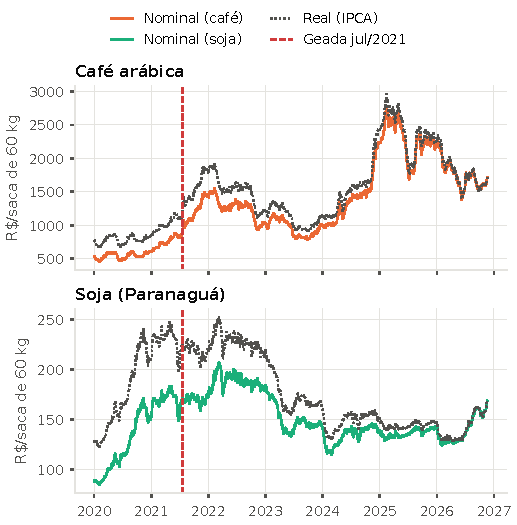
\includegraphics[width=\columnwidth]{p1_evolucao_precos.pdf}
\caption{P1: preço nominal e real (deflacionado pelo IPCA) do café arábica e da soja. A linha
tracejada marca a geada de 20/07/2021.}
\label{fig:p1}
\end{figure}

A Fig.~\ref{fig:p1} mostra trajetórias bem diferentes. O \textbf{café} passou de R\$~534 por saca em
janeiro de 2020 para R\$~1.709 em novembro de 2026, mais que o triplo. A média anual subiu de R\$~543
(2020) para R\$~966 (2021), ano em que o preço subiu 132\% de janeiro a dezembro. Depois recuou em
2022--2023 e explodiu em 2024 (+122\% no ano),
atingindo o recorde de R\$~2.769 em 2025. Em 2026 a média caiu para R\$~1.749, com queda de 21\% no ano.
A \textbf{soja} subiu 75\% ao longo de 2020, chegou ao pico de R\$~207 em 2022 e depois recuou, ficando entre
R\$~115 e R\$~146 em 2024 e voltando a R\$~169 no fim de 2026. Em termos reais (linha pontilhada), a soja
de 2024--2026 está abaixo do nível de 2020, enquanto o café continua bem acima.

\subsection{P2: Sazonalidade}

\begin{figure}[!tb]
\centering
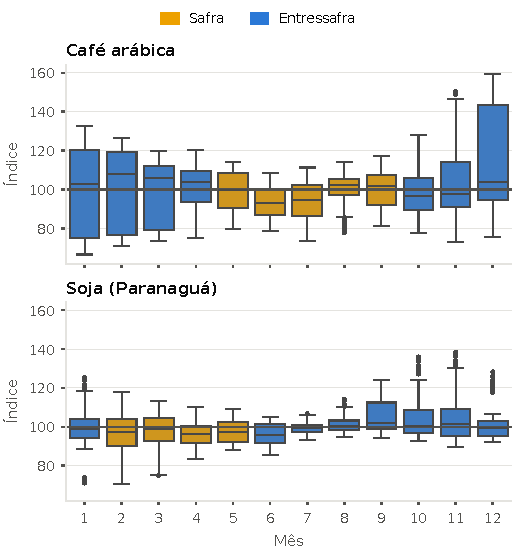
\includegraphics[width=\columnwidth]{p2_sazonalidade.pdf}
\caption{P2: preço real por mês, em índice (média do ano = 100); cores indicam safra e entressafra.}
\label{fig:p2}
\end{figure}

Para isolar o efeito sazonal da tendência, cada preço foi dividido pela média do seu ano
(Fig.~\ref{fig:p2}). O teste de Kruskal-Wallis rejeita a hipótese de meses iguais para os dois produtos
(café: $p\approx5\times10^{-14}$; soja: $p\approx6\times10^{-31}$). No \textbf{café}, os menores preços
relativos ocorrem em junho e julho (índice $\approx$94), no auge da colheita, e os maiores em dezembro
(113, com alta dispersão). Na \textbf{soja}, os preços ficam abaixo da média entre fevereiro e junho
(96--97), durante e logo após a colheita, e acima entre setembro e novembro (104--105), na entressafra. O
padrão é o esperado: mais oferta na safra, preço menor. A amplitude, porém, é pequena perto das grandes tendências da P1. Além disso, o teste supõe observações independentes, e dias seguidos têm preços parecidos; os $p$-valores parecem, portanto, mais fortes do que são.

\subsection{P3: Preço $\times$ dólar}

\begin{figure}[!tb]
\centering
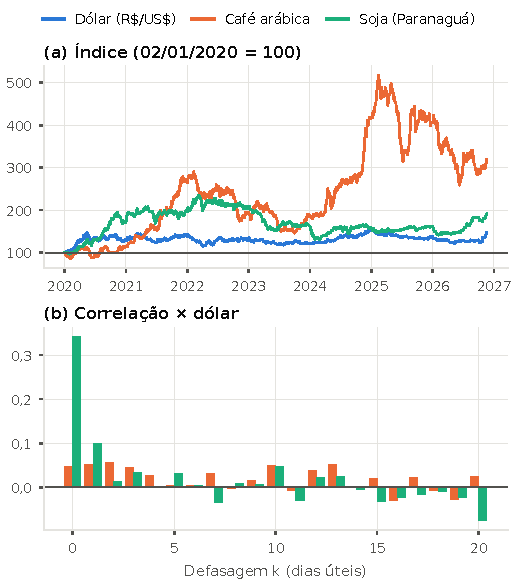
\includegraphics[width=\columnwidth]{p3_preco_dolar.pdf}
\caption{P3: (a) índices base 100; (b) correlação entre a variação diária do preço e a do
dólar $k$ dias úteis antes.}
\label{fig:p3}
\end{figure}

No índice base 100 (Fig.~\ref{fig:p3}a), o dólar oscila numa faixa estreita (100--150),
enquanto o café chega a 500, o que mostra que o câmbio sozinho não explica a alta do café. A correlação
cruzada das variações diárias (Fig.~\ref{fig:p3}b) separa os dois produtos: a \textbf{soja} responde ao dólar
\emph{no mesmo dia} ($\rho=0{,}34$, $p<10^{-47}$), um resíduo ainda aparece no dia seguinte (0,10) e
depois a correlação some. O \textbf{café} quase não responde no curto prazo (máximo de 0,06 com 2 dias de
defasagem). Na escala mensal, a regressão log-log das variações dá elasticidades parecidas (café 0,56;
soja 0,52, ou seja, cerca de metade da variação do dólar é repassada), mas o $R^2$ é baixo: o dólar explica
13,7\% da variação mensal da soja e apenas 5,3\% da do café.

\subsection{P4: Clima $\times$ preço do café}

\begin{figure}[!tb]
\centering
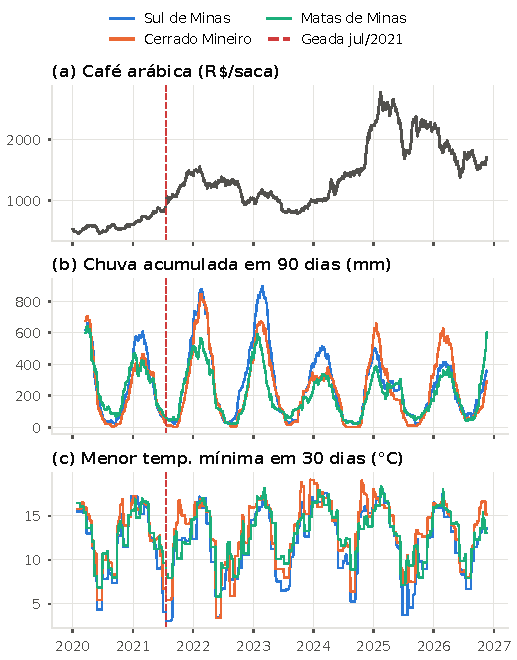
\includegraphics[width=\columnwidth]{p4_clima_regioes.pdf}
\caption{P4: preço do café, chuva acumulada em 90 dias e menor temperatura mínima em 30 dias nas três
regiões (NASA POWER).}
\label{fig:p4}
\end{figure}

A Fig.~\ref{fig:p4} mostra o ciclo regular de chuvas (verão úmido, inverno seco) e as quedas de
temperatura mínima no inverno, com o menor valor da série em julho de 2021. Para medir a relação
\emph{antecedente}, calculou-se a correlação de Spearman entre o clima no dia $t$ e a variação do preço nos
63 dias úteis seguintes ($\approx$3 meses). Para o café, as associações mais fortes vêm do
\textbf{Cerrado Mineiro}: a média das máximas em 30 dias ($\rho=+0{,}34$) e a chuva acumulada em 90 dias
($\rho=-0{,}26$), ambas com $p<10^{-25}$. Ou seja, \emph{períodos quentes e secos tendem a ser seguidos de
alta}, o que sugere uma resposta afirmativa à P4. As correlações são moderadas, os $p$-valores são otimistas porque as janelas de 63 dias se sobrepõem, e, como o clima é sazonal, parte
delas reflete o próprio calendário agrícola.

\subsection{P5: Geada de julho de 2021}

\begin{figure}[!tb]
\centering
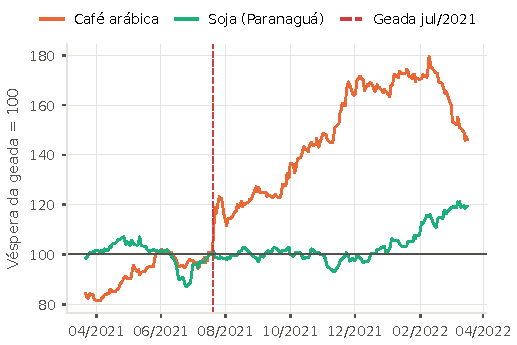
\includegraphics[width=\columnwidth]{p5_geada_2021.pdf}
\caption{P5: índices (véspera da geada = 100) do café e da soja; a soja, pouco cultivada nas regiões
afetadas, funciona como grupo de controle.}
\label{fig:p5}
\end{figure}

\begin{table}[!tb]
\centering
\caption{Variação do preço médio após a geada (em relação aos 30 dias anteriores)}
\label{tab:geada}
\small
\begin{tabular}{@{}lrrr@{}}
\toprule
Produto & 30 dias & 90 dias & 180 dias \\
\midrule
Café arábica & +20,9\% & +28,4\% & +46,9\% \\
Soja (Paranaguá) & +5,9\% & +6,3\% & +6,1\% \\
\bottomrule
\end{tabular}
\end{table}

A geada de 20/07/2021 é o caso mais claro de choque climático da série (Fig.~\ref{fig:p5}). O café
saltou quase 20\% nos dias seguintes, com duas das maiores altas diárias de toda a base, e continuou
subindo por meses, chegando a +80\% em fevereiro de 2022, já que a geada danificou a lavoura e afetou
também a safra seguinte. A média dos 180 dias seguintes foi 46,9\% maior que a dos 30 dias anteriores
(Tabela~\ref{tab:geada}), e o preço máximo foi de R\$~1.503, contra a média de R\$~840 antes da geada. A
soja, no mesmo período, variou cerca de 6\%, o que é compatível com um efeito climático e enfraquece a hipótese de um movimento geral de mercado ou de câmbio, embora não prove causalidade.

\subsection{P6: Sensibilidade ao clima e ao câmbio}

\begin{figure}[!tb]
\centering
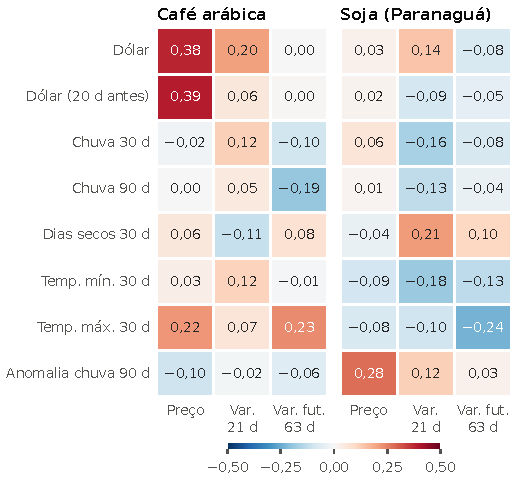
\includegraphics[width=\columnwidth]{p6_correlacoes.pdf}
\caption{P6: correlação de Spearman entre preço, variação em 21 dias e variação futura em 63 dias e as
variáveis de câmbio e clima (escala de cores de $-0{,}5$ a $0{,}5$).}
\label{fig:p6corr}
\end{figure}

\begin{figure}[!tb]
\centering
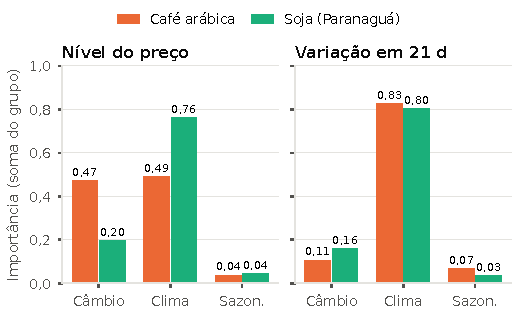
\includegraphics[width=\columnwidth]{p6_importancia_grupos.pdf}
\caption{P6: importância de cada grupo de atributos na \emph{Random Forest}.}
\label{fig:p6imp}
\end{figure}

\begin{table}[!tb]
\centering
\caption{Desempenho fora da amostra (média de 5 folds) e $R^2$ de ajuste}
\label{tab:modelos}
\small
\begin{tabular}{@{}llrrr@{}}
\toprule
Produto/alvo & Modelo & MAE & $R^2_{\text{teste}}$ & $R^2_{\text{ajuste}}$ \\
\midrule
Café, nível & Baseline & 532 & $-7{,}6$ & -- \\
            & Linear   & 595 & $-9{,}9$ & 0,32 \\
            & RF       & 624 & $-9{,}8$ & 0,98 \\
\addlinespace
Café, var.~21d & Baseline & 8,1 & $-0{,}27$ & -- \\
            & Linear   & 9,8 & $-0{,}70$ & 0,09 \\
            & RF       & 8,8 & $-0{,}40$ & 0,95 \\
\addlinespace
Soja, nível & Baseline & 23,1 & $-10{,}5$ & -- \\
            & Linear   & 28,1 & $-16{,}8$ & 0,35 \\
            & RF       & 23,0 & $-11{,}1$ & 0,98 \\
\addlinespace
Soja, var.~21d & Baseline & 3,9 & $-0{,}23$ & -- \\
            & Linear   & 4,8 & $-0{,}69$ & 0,19 \\
            & RF       & 4,8 & $-0{,}99$ & 0,93 \\
\bottomrule
\end{tabular}
\end{table}

As evidências são claras para o câmbio e mistas para o clima:
\begin{itemize}
  \item \textbf{A soja é mais sensível ao câmbio no curto prazo:} correlação diária com o dólar de 0,34,
  contra 0,05 do café, e $R^2$ cambial mensal de 13,7\%, contra 5,3\%;
  \item \textbf{O café parece mais sensível ao clima, com ressalvas:} após a geada, a alta em 180 dias foi quase oito vezes maior no café, mas a maior associação clima--preço futuro é parecida nos dois ($|\rho|=0{,}34$ no café e $0{,}30$ na soja). As correlações da soja com o clima mineiro podem ser espúrias, já que a soja de Paranaguá depende
  do clima do Centro-Oeste e do Sul, não do de Minas.
\end{itemize}

No nível de preço (Fig.~\ref{fig:p6corr}), o café tem correlação de 0,38 com o dólar, enquanto a soja
tem 0,03. Isso não contradiz o resultado diário: as duas séries subiram juntas na tendência de longo prazo
(correlação de nível), mas o café não reage às oscilações diárias do câmbio. Na \emph{Random Forest} para o
nível de preço (Fig.~\ref{fig:p6imp}), o câmbio responde por 47\% da importância no café e por apenas 20\% na soja, e o
clima, por 49\% e 76\%. A Tabela~\ref{tab:importancia} compara os dois modelos. Nos dois, o clima pesa mais na
soja quando o alvo é o nível e um pouco mais no café quando o alvo é a variação, de modo que os modelos
\emph{não confirmam} sozinhos a maior sensibilidade do café. Esses pesos pedem cautela: o clima tem sete
atributos, contra um a três do câmbio, e a soma favorece grupos maiores; o clima usado é só o de Minas; e os
modelos foram ajustados na série completa, com sobreajuste.

\begin{table}[!tb]
\centering
\caption{Importância por grupo: Linear (LR) e \emph{Random Forest} (RF)}
\label{tab:importancia}
\footnotesize
\setlength{\tabcolsep}{3.5pt}
\begin{tabular}{@{}lrrrrrr@{}}
\toprule
 & \multicolumn{2}{c}{Câmbio} & \multicolumn{2}{c}{Clima} & \multicolumn{2}{c}{Sazonalidade} \\
\cmidrule(lr){2-3}\cmidrule(lr){4-5}\cmidrule(l){6-7}
Produto/alvo & LR & RF & LR & RF & LR & RF \\
\midrule
Café, nível & 0,18 & 0,47 & 0,65 & 0,49 & 0,17 & 0,04 \\
Soja, nível & 0,10 & 0,20 & 0,70 & 0,76 & 0,20 & 0,04 \\
Café, var.~21d & 0,12 & 0,11 & 0,77 & 0,83 & 0,11 & 0,07 \\
Soja, var.~21d & 0,12 & 0,16 & 0,72 & 0,80 & 0,16 & 0,03 \\
\bottomrule
\end{tabular}
\end{table}

Quanto ao poder preditivo (Tabela~\ref{tab:modelos}), \emph{os modelos quase nunca superaram o baseline fora da amostra}, e todos os $R^2$ de teste são negativos. A exceção é o MAE da floresta no nível da soja (23,01 contra 23,13), com RMSE e $R^2$ piores. Com \texttt{TimeSeriesSplit}, cada \emph{fold} de teste
cai em um regime de preços que o treino nunca viu (por exemplo, o recorde de 2024--2025), e nenhum dos
modelos extrapola bem: a floresta não prevê valores fora do intervalo de treino, e a regressão
linear extrapola tendências que mudam de direção. Já o $R^2$ de ajuste alto da floresta (0,93--0,98)
contra o da regressão (0,09--0,35) indica sobretudo sobreajuste, já que não se repete fora da amostra. O
resultado está de acordo com o objetivo explicativo definido no pré-projeto: câmbio, clima e
sazonalidade ajudam a \emph{descrever} os movimentos, mas não bastam para prevê-los; fatores fora do estudo (estoques mundiais, produção de outros países, demanda) provavelmente também pesam.

\FloatBarrier
% =====================================================================
\section{Repositório}

Todo o projeto está no repositório público
\url{https://github.com/joaopaulocunhafaria/trabalho-fina-ciencia-dados}, organizado como segue:
\begin{itemize}\raggedright
  \item \texttt{src/coleta}: um módulo por fonte; \texttt{src/tratamento}: limpeza, integração, atributos
  e qualidade; \texttt{src/analise}: estatística e gráficos de P1--P6; \texttt{src/modelagem}: modelos;
  \texttt{src/pipeline.py}: orquestrador de todas as etapas;
  \item \texttt{data/raw}, \texttt{data/interim} e \texttt{data/processed}: dados brutos (nunca editados),
  limpos por fonte e integrados;
  \item \texttt{notebooks/}: 01 coleta e qualidade, 02 análise exploratória de P1--P6, 03 modelagem;
  \item \texttt{reports/}: figuras, tabelas, métricas e relatório de qualidade;
  \item \texttt{app/streamlit\_app.py}: painel interativo;
  \item \texttt{tests/}: 21 testes \texttt{pytest} dos \emph{parsers} (com páginas HTML salvas como
  \emph{fixtures}), do tratamento e da ausência de vazamento temporal nos atributos;
  \item \texttt{.github/workflows/crawler.yml}: coleta diária automática, com \emph{commit} dos novos dados.
\end{itemize}
A partir do repositório, que já inclui os dados brutos, usam-se \texttt{make venv}, \texttt{make tudo} e \texttt{make painel}. Para refazer a coleta do zero, é preciso ainda \texttt{make backfill} e baixar as planilhas do CEPEA.

% =====================================================================
\section{Alterações em relação ao pré-projeto}

\begin{itemize}
  \item \textbf{Histórico também pelo Notícias Agrícolas:} o CEPEA segue como fonte prioritária, mas bloqueia
  downloads automatizados e depende de planilhas manuais. O \emph{backfill} permitiu comparar as duas fontes
  em toda a série e completar os dias mais recentes;
  \item \textbf{Selenium não foi necessário:} as tabelas de cotação vêm no HTML estático, e
  \texttt{requests} + \texttt{BeautifulSoup} bastaram, com menor custo e mais estabilidade;
  \item \textbf{Ambiente local em vez do Google Colab:} \texttt{venv} + \texttt{Makefile} + GitHub tornam
  o projeto reprodutível e permitem a automação pelo GitHub Actions;
  \item \textbf{Inclusão de \texttt{yfinance}, \texttt{SciPy} e \texttt{pytest}:} para
  comparar preço interno $\times$ bolsa, fazer testes estatísticos e garantir que os \emph{parsers}
  continuem funcionando;
  \item \textbf{Índice base 100 em vez de eixo duplo} no gráfico de preço $\times$ dólar, pelo motivo citado
  na Seção~\ref{sec:visualizacao}.
\end{itemize}

% =====================================================================
\section{Conclusão e Considerações Finais}

O trabalho cumpriu os objetivos propostos: construiu, com coleta ética e automatizada, uma base
integrada e validada de quase sete anos sobre café, soja, câmbio e clima, e respondeu às seis perguntas de
pesquisa. Os principais resultados são: (i) o café mais que triplicou de preço no período, com dois grandes
ciclos de alta (2021 e 2024--2025), enquanto a soja subiu até 2022 e depois recuou; (ii) os dois produtos
apresentam padrão sazonal, com preços em geral menores na safra; (iii) a soja acompanha o dólar no
mesmo dia, enquanto o café quase não reage ao câmbio no curto prazo; (iv) períodos quentes e secos no
Cerrado Mineiro antecedem altas do café; (v) após a geada de 2021, o preço médio do café ficou quase 47\% maior em seis meses, contra 6\% da soja; e (vi) a soja é a mais sensível ao câmbio no curto prazo, enquanto a geada aponta o café como o mais sensível ao clima, o que os modelos não confirmam.

Como limitações, as relações encontradas são correlações e não causalidade, o clima de cada região
vem de um único ponto de grade, e variáveis importantes do mercado mundial não foram incluídas, o que pode contribuir para o baixo poder preditivo dos modelos. Como trabalhos futuros, sugere-se incluir dados de estoques,
de produção de outros países e do clima das regiões produtoras de soja, e testar modelos próprios de
séries temporais (ARIMAX, por exemplo). O \emph{crawler} está agendado para coletar novas cotações em cada dia útil.

% =====================================================================
\begin{thebibliography}{99}

\bibitem{conab}
Companhia Nacional de Abastecimento (Conab), ``Acompanhamento da safra brasileira de café,'' Brasília.
[Online]. Disponível: \url{https://www.conab.gov.br/info-agro/safras/cafe}

\bibitem{noticiasagricolas}
Notícias Agrícolas, ``Cotações.'' [Online]. Disponível:
\url{https://www.noticiasagricolas.com.br/cotacoes/}

\bibitem{cepea}
Centro de Estudos Avançados em Economia Aplicada (CEPEA/Esalq-USP), ``Indicadores de preços: café e
soja.'' [Online]. Disponível: \url{https://www.cepea.org.br/}

\bibitem{bcb}
Banco Central do Brasil, ``Sistema Gerenciador de Séries Temporais (SGS).'' [Online]. Disponível:
\url{https://www3.bcb.gov.br/sgspub/}

\bibitem{nasapower}
NASA, ``POWER -- Prediction Of Worldwide Energy Resources.'' [Online]. Disponível:
\url{https://power.larc.nasa.gov/}

\bibitem{inmet}
Instituto Nacional de Meteorologia (INMET), ``Dados históricos anuais.'' [Online]. Disponível:
\url{https://portal.inmet.gov.br/dadoshistoricos}

\bibitem{lgpd}
Brasil, ``Lei n\textordmasculine{} 13.709, de 14 de agosto de 2018 -- Lei Geral de Proteção de Dados Pessoais (LGPD).''
[Online]. Disponível: \url{https://www.planalto.gov.br/ccivil_03/_ato2015-2018/2018/lei/l13709.htm}

\bibitem{mitchell}
R. Mitchell, \emph{Web Scraping com Python: coletando mais dados da web moderna}, 2.~ed. São Paulo:
Novatec, 2019.

\bibitem{pandas}
W. McKinney, ``Data structures for statistical computing in Python,'' in \emph{Proc. 9th Python in Science
Conf.}, 2010, pp. 56--61.

\bibitem{sklearn}
F. Pedregosa \emph{et al.}, ``Scikit-learn: Machine learning in Python,'' \emph{J. Mach. Learn. Res.},
vol. 12, pp. 2825--2830, 2011.

\bibitem{breiman}
L. Breiman, ``Random forests,'' \emph{Machine Learning}, vol. 45, no. 1, pp. 5--32, 2001.

\bibitem{matplotlib}
J. D. Hunter, ``Matplotlib: A 2D graphics environment,'' \emph{Comput. Sci. Eng.}, vol. 9, no. 3,
pp. 90--95, 2007.

\bibitem{seaborn}
M. L. Waskom, ``seaborn: statistical data visualization,'' \emph{J. Open Source Softw.}, vol. 6, no. 60,
p. 3021, 2021.

\bibitem{airobots}
ai.robots.txt, ``A list of AI agents and robots to block.'' [Online]. Disponível:
\url{https://github.com/ai-robots-txt/ai.robots.txt}

\end{thebibliography}

\end{document}
